\documentclass[10pt,twocolumn,letterpaper]{article}

\usepackage{cvpr}
\usepackage{times}
\usepackage{epsfig}
\usepackage{graphicx}
\usepackage{amsmath}
\usepackage{amssymb}
\usepackage{booktabs}
\usepackage{microtype}
% From https://ctan.org/pkg/matlab-prettifier
\usepackage[numbered,framed]{matlab-prettifier}

\frenchspacing

% Include other packages here, before hyperref.

% If you comment hyperref and then uncomment it, you should delete
% egpaper.aux before re-running latex.  (Or just hit 'q' on the first latex
% run, let it finish, and you should be clear).
\usepackage[pagebackref=true,breaklinks=true,letterpaper=true,colorlinks,bookmarks=false]{hyperref}

\cvprfinalcopy % *** Uncomment this line for the final submission

\def\cvprPaperID{****} % *** Enter the CVPR Paper ID here
\def\httilde{\mbox{\tt\raisebox{-.5ex}{\symbol{126}}}}

% Pages are numbered in submission mode, and unnumbered in camera-ready
\ifcvprfinal\pagestyle{empty}\fi
\begin{document}

%%%%%%%%% TITLE
\title{CSCI 1430 Final Project Report:\\Your project title}

\author{\emph{Team name}: First member, second member, third member, fourth member.\\
Brown University\\
}

\maketitle
%\thispagestyle{empty}

%%%%%%%%% ABSTRACT
\begin{abstract}
This project analyzes and scores a poker hand given images of the hand. We trained a YOLOv3 object recognition model to detect and classify playing cards in images. We developed a variation of the Chen formula to score Texas Hold'em hands based on the likelihood of winning the hand.
\end{abstract}


% \section{Proposal Notes}

% \begin{enumerate}
%     \item Overriding principle: show us your effort.
%     \item If you wish us to consider any aspect of your project, it should be presented here. \item Please include a problem statement, related work, your method, your results (figures! tables!), any comparison to existing techniques, and references. 
%     \item If you made something work - great! If you didn't quite make it work - tell us about the problems, why you think it didn't work, and what you would do to fix it.
%     \item Please include an appendix to the report which details what each team member contributed to the project. One paragraph max each; not included in the 4-page limit.
%     \item Any other materials should go in an appendix. You can use more than 4 pages in this way.
% \end{enumerate}


%%%%%%%%% BODY TEXT
\section{Introduction}

We aimed to create an application that could evaluate a Texas Hold'em hand. To achieve this, we needed to train an object recognition model to accurately identify playing cards. We also had to develop an effective evaluation algorithm that gave a relevant score to hands. The algorithm also outputs the best hand out of all the cards available. We decided to use the YOLO (You Only Look Once) architecture for card detection. We augmented the Chen formula for scoring hands.

\section{Related Work}

Our work is inspired by the paper\textit{ Bridge bidding via playing card detection using YOLO v3} \cite{bridge}. We use YOLO object detection for its speed and accuracy in predicting object labels \cite{yolo}. Our scoring algorithm builds off of the \hyperlink{https://www.thepokerbank.com/strategy/basic/starting-hand-selection/chen-formula/}{ Chen Formula}, which scores two-card starting hands for Texas Hold'em. 

\section{Method}
\subsection{Data Set}

We utilized a data set generated by the authors of \textit{Bridge bidding via playing card detection using YOLO v3} (cite). The data set has 30,000 images of 2-3 playing cards against random background textures and xml files describing the metadata including bounding boxes. The data and steps to reproduce it can be found in the original paper \url{https://cs.brown.edu/research/pubs/theses/capstones/2020/xu.philip.pdf}. We pre-processed the images and XML files into the format needed by our network.

\subsection{Training}
We chose to use the YOLOv3 architecture to train a model that detects bounding boxes and class probabilities for objects in an image. YOLOv3 uses a fully connected convolutional network and splits an image into a grid, predicting all bounding boxes for each grid in a single pass. 

We used the Darknet framework to train the model. The Darknet model and code for generating other files required for training is available along with the rest of our project code at \url{https://github.com/bsmith175/poker-vision}. Instructions for training the model are available at \url{https://github.com/AlexeyAB/darknet}.

We trained the model with a batch size of 64 and a batch subdivision of 64, due to memory constraints. We used a 80/20 training/testing split. We trained the model for 72 hours and 9,000 iterations on NVIDIA Tesla K80. 

\subsection{Detection}

To perform detection in the application, we decided to use Python instead of Darknet for better extensibility and easier installation. With the help of \hyperlink{https://blog.paperspace.com/how-to-implement-a-yolo-object-detector-in-pytorch/}{this} tutorial, we created a PyTorch model that loads a Darknet YOLO model configuration and translates the model to PyTorch. We implemented a scoring/detection pipeline that can be given paths to images and outputs scores, bounding box and class predictions. 

\subsection{Scoring}
Discuss scoring algorithm here.

\section{Results}

The recognition model achieved a mAP (mean Average Precision) of 95.2\% on our 5,000 testing images. 
Here are some examples of the model's predictions on our testing data.
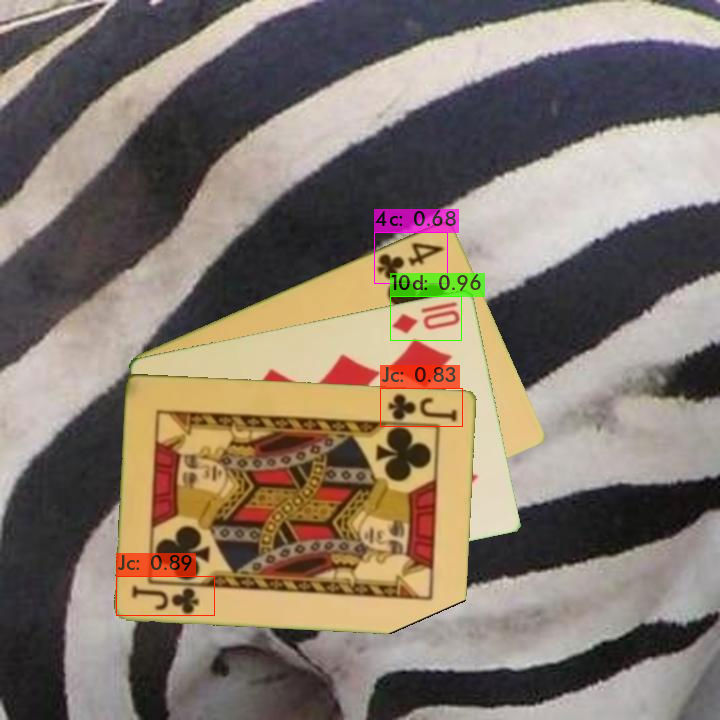
\includegraphics[width=4cm]{predictions (17).jpg}
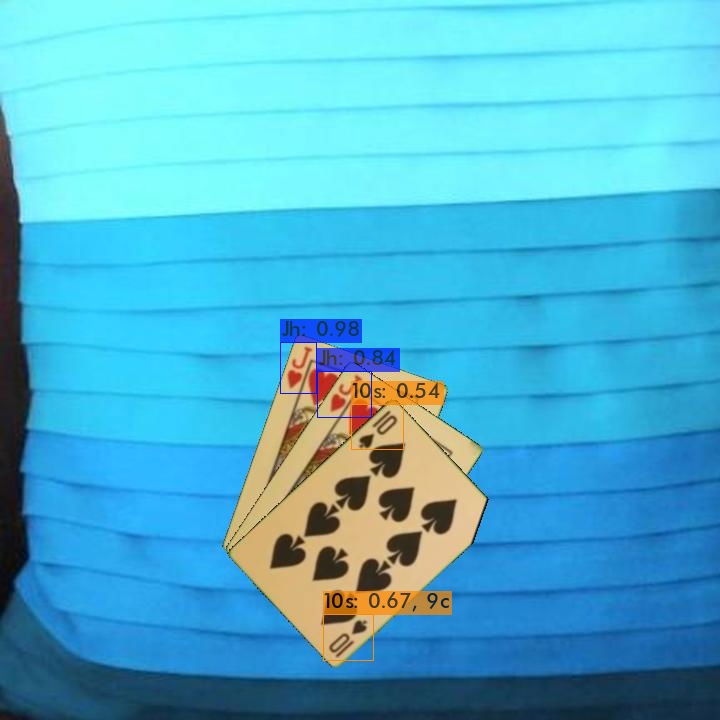
\includegraphics[width=4cm]{predictions (20).jpg}


%-------------------------------------------------------------------------
\subsection{Technical Discussion}

A higher accuracy should be possible to achieve. However, training was limited by compute resources and time, as we didn't expect the model to take several days to train. We experimented with using the Tiny YOLO3 architecture, which takes significantly less time per iteration. However, accuracy didn't seem to progress as much with this architecture, and with limited GCP credits and time to train, we decided to only fully train the original Yolo model. 

Our model performs significantly worse on hand taken images from different cameras. Possible explanations for this is that the dataset does not have variation in image resolution or angle. 


%-------------------------------------------------------------------------
\subsection{Societal Discussion}

Please respond to the following questions. Different projects will have different scales and qualities of impact; we ask you to think creatively and consider the broader implications of your project rather than just the more narrow current technical capability. Responses should together take up roughly one page in your final report.

\begin{enumerate}
\item Describe the socio-historical context of your project to identify three broad societal factors that could affect your data, goal, and/or hypothesis. These factors might include current or historical policies, events, social conditions, and larger societal systems. Cite at least one outside source.
 
\item Who are the major stakeholders in this project? What is your relationship to these stakeholders? \\
Stakeholders are those who may be affected by or have an effect on your project topic. Some examples of stakeholders are a particular demographic group, residents of a particular geographic area, and people experiencing or at risk for a particular problem.\\
Consider the following questions to help identify stakeholders:
    \begin{itemize}
    \item Who does this project topic currently affect?
    \item Who might be harmed by your research findings?
    \item Who might benefit from your research findings?
    \end{itemize}

\item Research or journalism on your broader project topic may have already been conducted. What was the societal impact of existing research? Discuss the implication of this research on your project and consider the following questions to help identify at least one implication. It may affect:
    \begin{itemize}
    \item How you should frame your goal,
    \item How you should design your algorithm,
    \item How you should analyze your data,
    \item How you should interpret your findings, and
    \item How you should present your results.
    \end{itemize}

\item How could an individual or particular community’s civil rights or civil liberties (such as privacy) be affected by your project?

\item If you are using data, what kind of biases might this data contain? Do any of these represent underlying historical or societal biases? How can this bias be mitigated? \\
    Consider the following questions to help you:
    \begin{itemize}
    \item Were the systems and processes used to collect the data biased against any groups?
    \item Is the data being used in a manner agreed to by the individuals who provided the data?
    \end{itemize}

\end{enumerate}

%------------------------------------------------------------------------
\section{Conclusion}

What you did, why it matters, what the impact is going forward.

{\small
\bibliographystyle{plain}
\bibliography{ProjectFinal_ProjectReportTemplate}
}

\section*{Appendix}

\subsection*{Team contributions}

Please describe in one paragraph per team member what each of you contributed to the project.
\begin{description}
\item[Person 1] Lorem ipsum dolor sit amet, consectetur adipiscing elit, sed do eiusmod tempor incididunt ut labore et dolore magna aliqua. Ut enim ad minim veniam, quis nostrud exercitation ullamco laboris nisi ut aliquip ex ea commodo consequat. Duis aute irure dolor in reprehenderit in voluptate velit esse cillum dolore eu fugiat nulla pariatur. 
\item[Person 2] Lorem ipsum dolor sit amet, consectetur adipiscing elit, sed do eiusmod tempor incididunt ut labore et dolore magna aliqua. Ut enim ad minim veniam, quis nostrud exercitation ullamco laboris nisi ut aliquip ex ea commodo consequat. Duis aute irure dolor in reprehenderit in voluptate velit esse cillum dolore eu fugiat nulla pariatur.
\item [Person 3] Lorem ipsum dolor sit amet, consectetur adipiscing elit, sed do eiusmod tempor incididunt ut labore et dolore magna aliqua. Ut enim ad minim veniam, quis nostrud exercitation ullamco laboris nisi ut aliquip ex ea commodo consequat. Duis aute irure dolor in reprehenderit in voluptate velit esse cillum dolore eu fugiat nulla pariatur. 
\item [Person 4] Lorem ipsum dolor sit amet, consectetur adipiscing elit, sed do eiusmod tempor incididunt ut labore et dolore magna aliqua. Ut enim ad minim veniam, quis nostrud exercitation ullamco laboris nisi ut aliquip ex ea commodo consequat. Duis aute irure dolor in reprehenderit in voluptate velit esse cillum dolore eu fugiat nulla pariatur.
\end{description}

\end{document}